\documentclass{article}
\usepackage[utf8]{inputenc}
\usepackage[spanish]{babel}
\usepackage{listings}
\usepackage{graphicx}
\graphicspath{ {images/} }
\usepackage{cite}


\begin{document}

\begin{titlepage}
    \begin{center}
        \vspace*{1cm}
            
        \Huge
        \textbf {Proyecto Final: Diseño y Planeación}
            
        \vspace{0.5cm}
        \LARGE
        Informática II
            
        \vspace{1.5cm}
            
        \textbf{Daniela Andrea Gallego Díaz\\ Manuela Gutiérrez Rodríguez }
            
        \vfill
            
        \vspace{0.8cm}
            
        \Large
        Despartamento de Ingeniería Electrónica y Telecomunicaciones\\
        Universidad de Antioquia\\
        Medellín\\
        12 de Octubre del 2021
            
    \end{center}
\end{titlepage}

\tableofcontents
\newpage

\section{Introducción} \label{Introducción}

\section{Modelamiento de objetos} \label{Modelamiento de objetos}

\subsection{Clases implementadas}

\subsubsection{Registro y validación de usuarios}

La clase permitirá la creación de diversos usuarios, los cuales serán identificados por un nombre de usuario y una contraseña única, para validar que la información ingresada sea correcta se buscará dentro de un documento txt y se verificará los datos. Una vez validado el usuario, la clase cargará el estado final en el que usuario dejó la partida, el cual se encuentra almacenado en otro documento txt, en caso de que el usuario sea nuevo, empezará en el primer nivel. También permite guardar la partida y actualizar dicho documento.

\subsubsection{Personajes Principales}

Esta clase contará con métodos y atributos para dos personajes, cada uno con diferentes diseños (basados en Robin Hood). Los dos personajes serán contrincantes por lo que solo ganará el que llegue primero a la puerta y tenga la llave en su poder, además de acumular puntos. Cada personaje contará con métodos para identificar colisiones y hacer diferentes acciones dependiendo del objeto con el que colisionan, también contarán con movimientos parabólicos al saltar y desplazarse por el escenario, además de contar con sprites para mejor estética del juego y fluidez en los movimientos. Cabe mencionar que los personajes tendrán la capacidad de tirar flechas para derrotar a sus enemigos y conseguir las llaves, cada vez que derroten a un enemigo acumularan puntos, así como también cuando avancen entre niveles. El jugador que acumule más puntos para el final del juego será el ganador definitivo. (Véase las interacciones entre la clase personaje). Hay que aclarar que además de derrotar a sus enemigos y encontrar la llave para abrir la puerta los jugadores tienen la misión de resolver el laberinto para así poder llegar a la puerta y pasar de nivel además de esquivar los ataques de sus enemigos, si el jugador se deja alcanzar del fuego escupido por enemigo perderá una de sus tres vidas y también se le restaran puntos.

\subsubsection{Enemigos}

 En esta clase, se contará con el diseño de un personaje que debe enfrentarse a los protagonistas. A medida que se sube de nivel, su resistencia a las flechas (véase clase flechas) será mayor, estas flechas causarán daño al enemigo y cuando el número de éstas sea suficiente, el enemigo morirá. Por otra parte, en cada nivel existirá un enemigo especial, debido a que cuando éste muera, soltará la llave maestra (véase clase llave). Su método de defensa será la posibilidad de escupir fuego, hiriendo a los personajes principales. Respecto a los modelamientos físicos se utilizará el movimiento parabólico para saltar y esquivar algunas flechas y el movimiento rectilíneo uniforme para desplazarse a través del escenario, el fuego que éste suelta se moverá con movimiento parabólico para una caída más natural. Los sprites serán parte secundaria del diseño, estos darán la impresión de desplazamiento y se ubicarán de acuerdo a la dirección del movimiento del enemigo.

\subsubsection{Flecha}

 Los jugadores utilizarán las flechas para infringir daño a sus enemigos, para ello la clase contará con métodos para el modelamiento de los movimientos parabólicos que harán las flechas al ser disparadas, además de identificar colisiones entre las flechas y los enemigos y así poder derrotarlos. La flecha desaparecerá en cuanto derrote al enemigo o caiga al suelo en caso de fallar. Cabe aclarar que cada vez que se derrote al enemigo se acumularan puntos para el jugador.
 

\subsubsection{Llave}

La llave estará en poder de uno de los enemigos aleatoriamente, por lo que los personajes tendrán que derrotar a varios enemigos para encontrarla, para ello, la clase contará con un método para elegir a uno de los enemigos aleatoriamente y ocultar la llave con el. También habrá un método para identificar las colisiones, por ejemplo cuando uno de los personajes principales derrote al enemigo se mostrará la llave y estará en poder del personaje que la halló, además de que cuando la llave colisione con la puerta se muestre el letrero para pasar al siguiente nivel. También se darán puntos extra por encontrar la llave.


\subsubsection{Puerta}

 La puerta será la entrada al siguiente nivel y solo se abrirá si el jugador tiene la llave en su poder, cabe mencionar que la puerta está ubicada en medio del laberinto. Esta clase contará con métodos para identificar las colisiones con la llave y el personaje para así pasar de nivel. Hay que aclarar que cuando se avanza de nivel el laberinto se hace más difícil de resolver, por lo que no será tan sencillo para los jugadores encontrar la puerta.


\subsubsection{Resorte}

Este resorte se ubicará en un espacio determinado del escenario y se activará cada cierto tiempo, en caso de que alguno de los personajes o enemigos se encuentre cerca, este será empujado debido a la energía potencial elástica del resorte comprimido. Su función principal es comprimirse y descomprimirse cada cierto tiempo, por lo que los jugadores deben tener cuidado de no ser desplazados por éste. La fuerza que realiza el resorte está dictada por la ley de hooke.

\subsubsection{Pared}

Consiste en un rectángulo que tiene una ubicación específica dentro del escenario, esta no tiene movimiento. Gracias a esta clase es que se pueden crear los laberintos, debido a que se hace un arreglo de paredes y se ubican según el diseño del escenario.


\subsection{Interacción entre clases}

\subsubsection{Interacción personajes-pared}

Constantemente se está evaluando colisiones entre estos dos, en caso de que exista el personaje va a tener un movimiento de tipo rebote, para de este modo, evitar que el personaje atraviese las paredes. De igual forma esto se realiza con los enemigos, cada vez que uno de ellos colisione se cambia su dirección de movimiento.

\subsubsection{Interacción personajes-enemigos}

Cuando exista una colisión entre ellos, será de tipo inelástica, por lo que conservarán su momento lineal. Por otra parte, cuando alguno de los enemigos esté en modo ofensivo y saque fuego, en caso de que el fuego colisione con los personajes, estos reducirán su vida.

\subsubsection{Interacción personajes/enemigos-resorte}

Debido a que el resorte realiza un movimiento periodico, el desplazamiento de los personajes es efectuado cuando alguno de ellos colisione con la parte frontal del resorte, el desplazamiento depende de si el resorte se encuentra comprimido o no, ya que a partir de esto el personaje tendrá una velocidad mayor o menor, según el caso.

\subsubsection{Interacción llave-puerta}

Cuando la llave colisione con la puerta, ésta se abrirá y saldrá un aviso diciendo al usuario que ha superado el nivel.


\subsubsection{Interacción llave-enemigos}

Un enemigo especial será el encargado de portar la llave, cuando el enemigo muera, éste desaparecerá del escenario e inmediatamente en la posición en la cual se encontraba aparecerá la llave, es decir, las últimas coordenadas del enemigo serán las que van a indicar la posición inicial de la llave.


\subsubsection{Interacción llave-personaje}

Una vez alguno de los personajes colisione con la llave, ésta se moverá en la misma dirección y con igual velocidad que el personaje, para dar la impresión de que el personaje lleva la llave consigo.


\subsubsection{Interacción flechas-enemigos}

Los enemigos solo serán derrotados una vez que la flecha colisione con ellos, cuando esto pase se acumularan puntos al jugador que haya asesinado a un enemigo e inmediatamente al colisionar la flecha con el enemigo, ambos (la flecha y el enemigo derrotado) desaparecen del escenario. 


\section{Cronograma} \label{Cronograma}

\begin{figure}[h!]
    \centering
    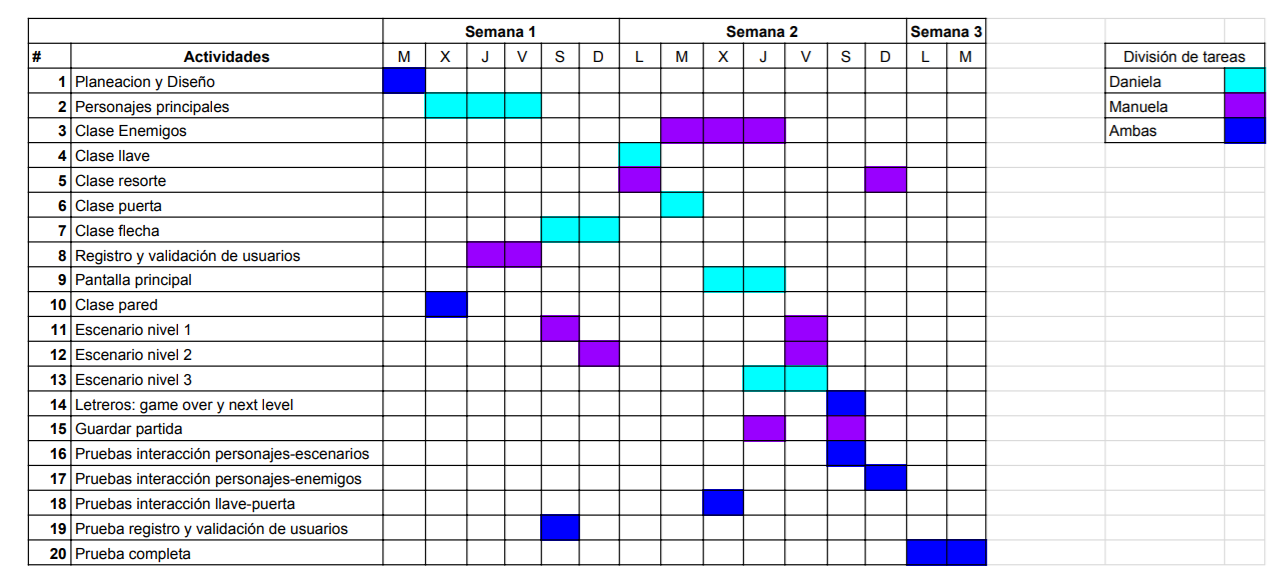
\includegraphics[scale=0.5]{IdeaFinal/images/Cronograma.png}
\end{figure}




\end{document}
